\documentclass[../main.tex]{subfiles}

\begin{document}
	
\subsection{Исследование поведения алгоритма в зависимости от изменяемых параметров}
	
	Рассмотрим формулу
	\begin{equation*}
		\begin{matrix}
		P_{ij,k}(t) & = 
		& \left\{
			\begin{matrix}
			0, & \mbox{ } j \notin J_{i,k} \\
			\frac {(τ_{ij}(t))^\alpha * (η_{ij})^\beta} {\sum \limits_{q \in J_{i,k}} (τ_{iq}(t))^\alpha * (η_{iq})^\beta}, & \mbox{ } j \in J_{i,k}. \\
			\end{matrix} \right.
		\end{matrix}
	\end{equation*}
	
	Её результатом будет являться вероятность, которая не будет превышать значение, равное единице. 
	Обеспечивается это тем, что внизу стоит сумма произведений для всех граней, а сверху - только для одной, входящей в сумму знаменателя.
	
	Как было указано в аналитическом разделе, формула обладает двумя регулируемыми параметрами:\\
	$\alpha$ - значимость для муравья феромона, оставленного на путях; \\
	$\beta$ - важность расстояния до конкретного города.\\
	Если отрегулировать данные параметры, можно добиться разной эффективности работы алгоритма.
	
	В частности, если, к примеру, $\alpha = 0$, то алгоритм из муравьиного вырождается в жадный алгоритм, то есть муравей игнорирует опыт предыдущих агентов и просто выбирает самое кратчайшее ребро из всех возможных. 
	Минусом такого выбора может являться то, что нет гарантии, что такой путь даст наилучшее решение, поскольку у более длинного ребра дальнейший путь может оказаться короче, чем тот, который получится по сделанному муравьём выбору.
	
	Если же принять $\beta = 0$, то муравей игнорирует расстояние и руководствуется лишь феромоном, оставленным на путях. 
	В таком случае алгоритм не зависит от конкретного расположения городов вообще, то есть характер его работы случайный, а результат непредсказуемый, что может дать в конкретных ситуациях такое решение, которое окажется хуже результата в случае превращения алгоритма в жадный.
	
	Важно понимать, что нельзя слишком большую роль отводить случайности, а именно это и регулирует параметр $\beta$. 
	Случайность в алгоритме должна лишь давать шанс на то, что будет выбран не самый оптимальный на первый взгляд путь, который может быть самым кратчайшим в дальнейшей перспективе.
	
	Из данных соображений можно сделать вывод, что необходимо всегда устанавливать более значимым параметр $\beta$, однако М.Дориго, автор алгоритма, утверждает, что наилучший результат достигается при $\alpha = \beta$.
	
	На феромон оказывает влияние параметр ρ - коэффициент испарения феромона:
	\begin{equation*}
		τ_{ij}(t+1) = (1-ρ) * τ_{ij}(t) + \sum \limits_{k=1}^m \Delta τ_{ij,k}(t).
	\end{equation*}
	
	Если $ρ = 0$, то феромон не испаряется вообще. Построим рассуждения следующим образом:
	\begin{enumerate}
		\item в самом начале количество феромона везде одинаково, вероятнее всего то, что муравей пойдёт к самому ближайшему городу; 
		
		\item так как феромон не испарялся, перевес ближайшего города начинает увеличиваться;
		
		\item как итог, все муравьи будут выбирать кратчайшее ребро из доступных, следовательно, будет получена версия жадного алгоритма.
	\end{enumerate}

	Если $ρ = 1$, то испаряется весь феромон, а это значит, что роль предыдущих поколений сводится к нулю. Теряется сам смысл муравьиного алгоритма - опора на опыт предыдущих агентов.
	
	В результате, можно прийти к выводу, что испарение не должно принимать крайних значений, находясь между ними. Вероятно, оптимальным значением может быть $ρ \approx 0.5$, которое может несколько увеличиваться или уменьшаться, но при большом отклонении значения к крайним есть потенциальная вероятность вырождения алгоритма в жадный или вероятность потери опоры на опыт других поколений.
	
\subsection{Характеристики оборудования}
	
	\begin{enumerate}[1)]
		\item Компьютер:
		\begin{enumerate}
			\item Тип компьютера   Компьютер с ACPI на базе x64;
			\item Операционная система   Microsoft Windows 10 Pro.
		\end{enumerate}
		\item Системная плата:
		\begin{enumerate}
			\item тип ЦП   DualCore Intel Core i5-6200U, 2700 MHz (27 x 100);
			\item системная плата   HP 8079;
			\item чипсет системной платы   Intel Sunrise Point-LP, Intel Skylake-U;
			\item системная память   8072 МБ (DDR4 SDRAM).
		\end{enumerate}
	\end{enumerate}

\subsection{Пример работы}

	Для тестирования и оценки параметров был выбран граф, представленный на рисунке \ref{graph2.6} и заданный следующей матрицей (первая строка и первый столбец задают города, пересечения их элементов задают расстояние между городами, если между ними есть прямой путь):
	
	\begin{figure}[H]
		\centering
		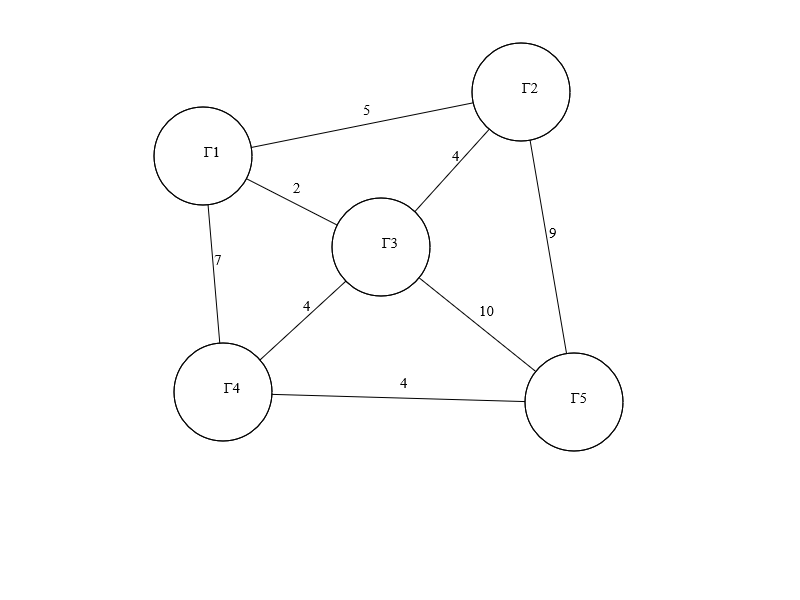
\includegraphics[scale=0.5]{src/img/4}
		\caption{}
		\label{fig:4}
	\end{figure}
	
	\begin{table}[ht]
		\caption{Матрица расстояний между городами}
		\begin{tabular}{|l|c|c|c|c|c|}
			\hline
			& Г1 & Г2 & Г3 & Г4 & Г5\\
			\hline
			\hline
			Г1 & 0 & 5 & 2  & 7 &  0\\
			\hline
			Г2 & 5 & 0 & 4 & 0 & 9\\
			\hline
			Г3 & 2 & 4 & 0 & 4 & 10\\
			\hline
			Г4 & 7 & 0 & 4 & 0 & 4\\
			\hline
			Г5 & 0 & 9 & 10 & 4 & 0\\
			\hline
		\end{tabular}
		\label{tab:tabular}
	\end{table}

	Для данной матрицы лучший путь, обнаруженный муравьиной колонией, составлял 17. \\
	
	Нахождение решение перебором обнаружило результат, равный 15.
	
	\begin{table}[H]
		\caption{Время работы алгоритмов}
		\begin{tabular}{|l|c|c|c|}
			\hline
			Время жизни колонии & Перебор & Муравьи & Разница времени работы в процентах\\
			\hline
			\hline
			1 & 0.000223 & 0.000168 & -33\%\\
			\hline
			10 & 0.000249 & 0.001213 & +21\%\\
			\hline
			100 & 0.000282 & 0.012529 & +98\%\\
			\hline
			1000 & 0.000238 & 0.127736 & +193\%\\
			\hline
			10000 & 0.000222 & 1.216264 & +292\%\\
			\hline
		\end{tabular}
		\label{tab:tabular}
	\end{table}

	На графике \ref{graph4.1} представлена зависимость средних значений длины пути при времени жихни колонии на выборках от 1 до $10^4$ от параметров $\alpha$ и ρ (параметр $\beta$ связан со значением $\alpha$, поэтому на графике не рассматривается отдельно).
	
	\pgfplotsset{compat=1.9}
	\pgfplotsset{Param/.style = {blue, samples = 100}}
	\begin{figure}
		\begin{tikzpicture}
		\begin{axis}[zlabel=Средняя длина пути, ylabel=ρ, xlabel=$\alpha$, width = 15cm, xmin = 0, ymin = 0, legend pos = north west]
		\legend{Зависимость от параметров}
		\addplot3[Param] table {
			x            y            z
			0           0            19.2
			0           0.2         17.4
			0           0.4         17.0
			0           0.6         18.6
			0           0.8         18.6
			0           1            17.8
			0.2        0            18.4
			0.2        0.2         18.0
			0.2        0.4         18.0
			0.2        0.6         17.4
			0.2        0.8         20.0
			0.2        1            18.2
			0.4        0            18.0
			0.4        0.2         18.6
			0.4        0.4         17.8
			0.4        0.6         19.0
			0.4        0.8         18.6
			0.4        1            18.2
			0.6        0            18.2
			0.6        0.2         20.2
			0.6        0.4         17.4
			0.6        0.6         18.4
			0.6        0.8         19.0
			0.6        1            19.2
			0.8        0            18.2
			0.8        0.2         18.6
			0.8        0.4         18.6
			0.8        0.6         18.2
			0.8        0.8         17.4
			0.8        1           17.4
			1           0           17.8
			1           0.2        18.0
			1           0.4        18.2
			1           0.6        17.8
			1           0.8        17.0
			1           1           17.8
		};
		\end{axis}
		\end{tikzpicture}
		\caption{График зависимостей параметров $\alpha$, ρ и среднего значения найденного пути за всё время жизни колонии при данных параметрах}
		\label{graph4.1}
	\end{figure}
	
	На рисунке \ref{graph2.7} представлены средние значения с помощью поверхностной диаграммы.
	
	\begin{table}[ht]
		\caption{Наборы параметров при стабильном результате}
		\begin{tabular}{|l|c|c|c|c|}
			\hline
			Набор & $\alpha$ & $\beta$ & ρ\\
			\hline
			\hline
			1 & 0 & 1 & 0.4 \\
			\hline
			2 & 1 & 0 & 0.8 \\
			\hline
		\end{tabular}
		\label{tab:tabular}
	\end{table}
	
	Наборы параметров, при которых алгоритм постепенно увеличивает длину найденного пути:
	
	\begin{table}[ht]
		\caption{Наборы параметров при увеличении длины пути}
		\begin{tabular}{|l|c|c|c|c|}
			\hline
			Номер набора & $\alpha$ & $\beta$ & ρ\\
			\hline
			\hline
			1 & 0.2 & 0.8 & 0.2 \\
			\hline
			2 & 0.2 & 0.8 & 0.4 \\
			\hline
			3 & 1 & 0 & 0.6 \\
			\hline
		\end{tabular}
		\label{tab:tabular}
	\end{table}
	
	Наборы параметров, при которых алгоритм позволяет постепенно снижать длину найденного пути:
	
	\begin{table}[ht]
		\caption{Наборы параметров при уменьшении длины пути}
		\begin{tabular}{|l|c|c|c|c|}
			\hline
			Номер набора & $\alpha$ & $\beta$ & ρ\\
			\hline
			\hline
			1 & 0 & 1 & 0 \\
			\hline
			2 & 0.2 & 0.8 & 1 \\
			\hline
			3 & 0.4 & 0.6 & 0 \\
			\hline
			4 & 0.4 & 0.6 & 1 \\
			\hline
			5 & 0.6 & 0.4 & 0 \\
			\hline
			6 & 0.8 & 0.2 & 1 \\
			\hline
		\end{tabular}
		\label{tab:tabular}
	\end{table}

	Набор параметров, рассматриваемых в гипотезе, заявленной в аналитическом разделе ($\alpha = 0.5, \beta = 0.5, ρ = 0.5$), при любом времени жизни колонии из рассматриваемого промежутка (от 1 до 10000) даёт минимальный путь из находимых муравьиным алгоритмом для данного примера, то есть 17. Результат остаётся аналогичным и в том случае, если при том же значении коэффициента испарения феромона параметры $\alpha = [0.4..0.5], \beta = [0.5..0.6]$.
	
\subsection{Вывод}

	В результате экспериментов подтвердилось то, что оптимальной является ситуация, когда $\alpha = 0.5, \beta = 0.5, ρ = 0.5$. Если параметры $\alpha$ и $\beta$ позволяли изменить их в противоположные стороны вплоть до $\Delta0.1$ относительно уравновешенного значения, то параметр ρ увеличивал найденную длину пути даже при изменении на 10\% в любую из сторон. \\
	
	Стабильное изменение результатов работы (в том числе, постоянный результат при различных значениях времени жизни из выборки) муравьиной колонии на неориентированном графе сопровождалось тем, что параметры начинали вырождаться.
	
\end{document}